\section{Digitale Bildverarbeitung in Matlab}
\subsection{Mathematische Beschreibung von Bildern}
Nach der Abtastung und Diskretisierung eines Bildes liegt die Bildinformation in Form eines
orts- und wertdiskreten Signals im Speicher vor. Das Grauwertbild lässt sich so durch eine
zweidimensionale Funktion darstellen. Die Werte der Funktion beschreiben Graustufen im
Bereich von 0 (schwarz) bis 255 (weiß), was einer Auflösung von 8 Bit entspricht.

\begin{align}
g_{min}=&\, 0  \leq g(i,j) \leq 255 = g_{max}\\
i:&\, \text{Nummer der Spalte}\nonumber\\
j:&\, \text{Nummer der Zeile}\nonumber
\end{align}

\noindent Hier ein einfaches Beispielbild und die dazugehörige Bildmatrix:

\begin{figure}[htbp]
	\centering
	\fbox{
\includegraphics[width=0.24\textwidth]{img/bildverarbeitung/Schachbrett_16x10.png}}
	\caption{Zweier"=Schachbrett mit $16 \times 10$ Pixeln und $8$ Bit Auflösung}\label{schachbrett1}
	\label{fig:schachbrett}
\end{figure}

\begin{figure}[htbp]
	\centering
	{\small 
		${ D_1=}
		\left(
\setstretch{1.3}\begin{array}{cccccccccccccccc}
		0&0&255&255&0&0&255&255&0&0&255&255&0&0&255&255\\ 
		0&0&255&255&0&0&255&255&0&0&255&255&0&0&255&255\\
		255&255&0&0&255&255&0&0&255&255&0&0&255&255&0&0\\
		255&255&0&0&255&255&0&0&255&255&0&0&255&255&0&0\\
		0&0&255&255&0&0&255&255&0&0&255&255&0&0&255&255\\
		0&0&255&255&0&0&255&255&0&0&255&255&0&0&255&255\\
		255&255&0&0&255&255&0&0&255&255&0&0&255&255&0&0\\
		255&255&0&0&255&255&0&0&255&255&0&0&255&255&0&0\\
		0&0&255&255&0&0&255&255&0&0&255&255&0&0&255&255\\
		0&0&255&255&0&0&255&255&0&0&255&255&0&0&255&255\\
		\end{array}
		\right)$} \caption{Helligkeitsmatrix $D_1$ zu Abb.
		\ref{schachbrett1}}
	\label{fig:matrix}
\end{figure}

\subsection{Farbvergrauung}

Die Farbvergrauung dient dazu, farbige Bilder in Grauwertbilder zu überführen. Dies führt zu einer Reduktion der Datenmenge pro Bild auf ein Drittel (wenn keine Komprimierung vorliegt), da die drei Kanäle für jeweils rot, grün und blau bei Farbbildern auf lediglich einen bei Grauwertbildern reduziert wird.\newline
Die Farbvergrauung ist dabei immer verlustbehaftet, da $16~777~216$ ($256 \cdot 256 \cdot 256$) Farben auf lediglich $256$ Grauwerte abgebildet werden.

Es werden hier vier Methoden vorgestellt, die sich darin unterscheiden, wie aus den drei Farbwerten pro Pixel der entsprechende Grauwert berechnet wird.\newline
Im Folgenden beschreibt $g(i,j,f)$ ein Pixel eines Farbbildes, wobei $f$ für den entsprechenden Farbkanal -- rot ($f=1$), grün ($f=2$) oder blau ($f=3$) -- steht. 
\begin{enumerate}
	\item \textbf{Einkanalmethode} \newline
	Bei diesem Verfahren wird lediglich ein Kanal (rot, grün oder blau) in Betracht gezogen, indem einfach dessen Wert als neuer Grauwert interpretiert wird.
	\begin{equation}
	g(i,j)=g(i,j,f)\;\forall\,i,j\;\text{und}\; f = \text{const.} \in\left\lbrace 1,2,3\right\rbrace 
	\end{equation}
	
	\item \textbf{Maximalwertmethode} \newline
	Hierbei wird der Maximalwert aller drei Farbkanäle als neuer Grauwert gesetzt.
	\begin{equation}
	g(i,j)=max\left\lbrace g(i,j,f):f\in\left\lbrace 1,2,3\right\rbrace \right\rbrace \;\forall\,i,j 
	\end{equation}
	\item \textbf{Mittelwertmethode} \newline
	Bei der Mittelwertmethode setzt man den Grauwert des neuen Bildes auf das arithmetische Mittel aus allen drei Farbwerten. 
	\begin{equation}
	g(i,j)=\frac{g(i,j,1)+g(i,j,2)+g(i,j,3)}{3}\;\forall\,i,j
	\end{equation}
	\pagebreak
	\item \textbf{Root of Mean Square (RMS)} \newline
	Hierbei nutzt man die aus der Fehleranalyse bekannte Formel zur Berechnung eines Mittelwertes aus der Summe der Quadrate der Einzelelemente, geteilt durch die Anzahl der Elemente.
	\begin{equation}
	g(i,j)=\sqrt{\frac{g(i,j,1)^{2}+g(i,j,2)^{2}+g(i,j,3)^{2}}{3}}\;\forall\,i,j
	\end{equation}
\end{enumerate}

Wie die resultierenden Bilder bei den verschiedenen Farbvergrauungsmethoden aussehen, ist beispielhaft in Abbildung~\ref{fig:farbvergrauung} dargestellt.

\begin{figure}[h]
	\centering
	\begin{tabular}{cccc}
		Original & nur roter Kanal & nur grüner Kanal & nur blauer
		Kanal\\
		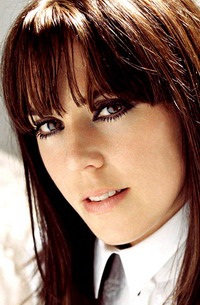
\includegraphics[scale=.43]{img/bildverarbeitung/melcrgb.jpg}&
		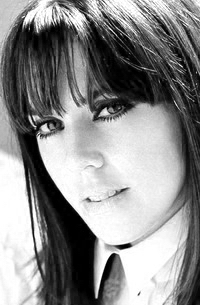
\includegraphics[scale=.43]{img/bildverarbeitung/melc_channel_red.jpg}&
		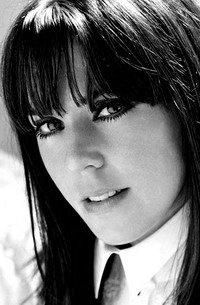
\includegraphics[scale=.43]{img/bildverarbeitung/melc_channel_green.jpg}&
		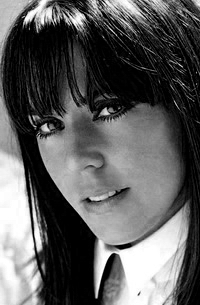
\includegraphics[scale=.43]{img/bildverarbeitung/melc_channel_blue.jpg}\\
		\midrule
		Adobe Photoshop & Maximum aller Kanäle & Mittelwert & Mean Square\\
		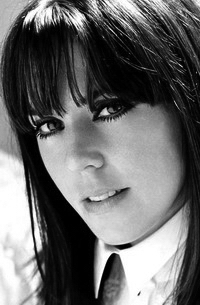
\includegraphics[scale=.43]{img/bildverarbeitung/melcgrey_adobe.jpg}&
		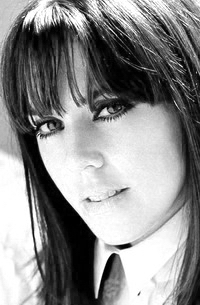
\includegraphics[scale=.43]{img/bildverarbeitung/melc_max.jpg}&
		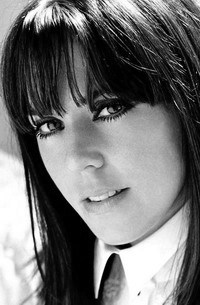
\includegraphics[scale=.43]{img/bildverarbeitung/melc_mean.jpg}&
		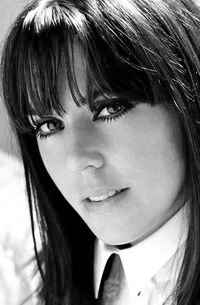
\includegraphics[scale=.43]{img/bildverarbeitung/melc_mean_square.jpg}
	\end{tabular}
	\caption[Farbvergrauung am Beispiel von Mel C]{Farbvergrauung am Beispiel von Mel C. Als Referenz dient das Ergebnis der kommerziellen Software \textit{Adobe Photoshop}. }
	\label{fig:farbvergrauung}
\end{figure}

\clearpage

\subsection{Histogramm}
In der digitalen Bildverarbeitung wird unter einem Histogramm die statistische
Häufigkeit der Grauwerte bzw. der Farbwerte in einem Bild verstanden. Das Histogramm eines Bildes
erlaubt eine Aussage über die vorkommenden Grau- bzw. Farbwerte und über Kontrastumfang
und Helligkeit des Bildes. In einem farbigen Bild kann entweder ein Histogramm über alle
möglichen Farben oder drei Histogramme über die einzelnen Farbkanäle erstellt werden. Letzteres ist meist sinnvoller, da die meisten Verfahren auf Grauwertbildern basieren
und so die sofortige Weiterverarbeitung möglich ist.
Ein Histogramm visualisiert somit die Verteilung der Helligkeitswerte eines Bildes. Über einer
Achse, die den Wertebereich der Farb- bzw. Grauwerte darstellt, sind als Balken die einzelnen
Häufigkeiten des Vorkommens der Farbwerte aufgetragen. Je höher der Balken über einem
Farbwert ist, desto häufiger kommt dieser Farbwert im Bild vor (Abbildung \ref{melchisto}).
\begin{figure}[htbp]
	\centering
	\begin{tabular}{cc}
		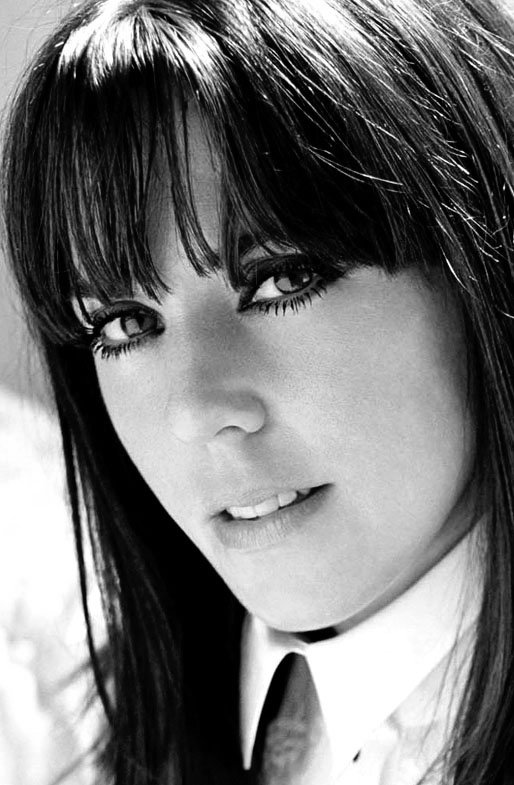
\includegraphics[scale=.19]{img/bildverarbeitung/melanie-c-1600x1200_gsc_v1.jpg}
		&
		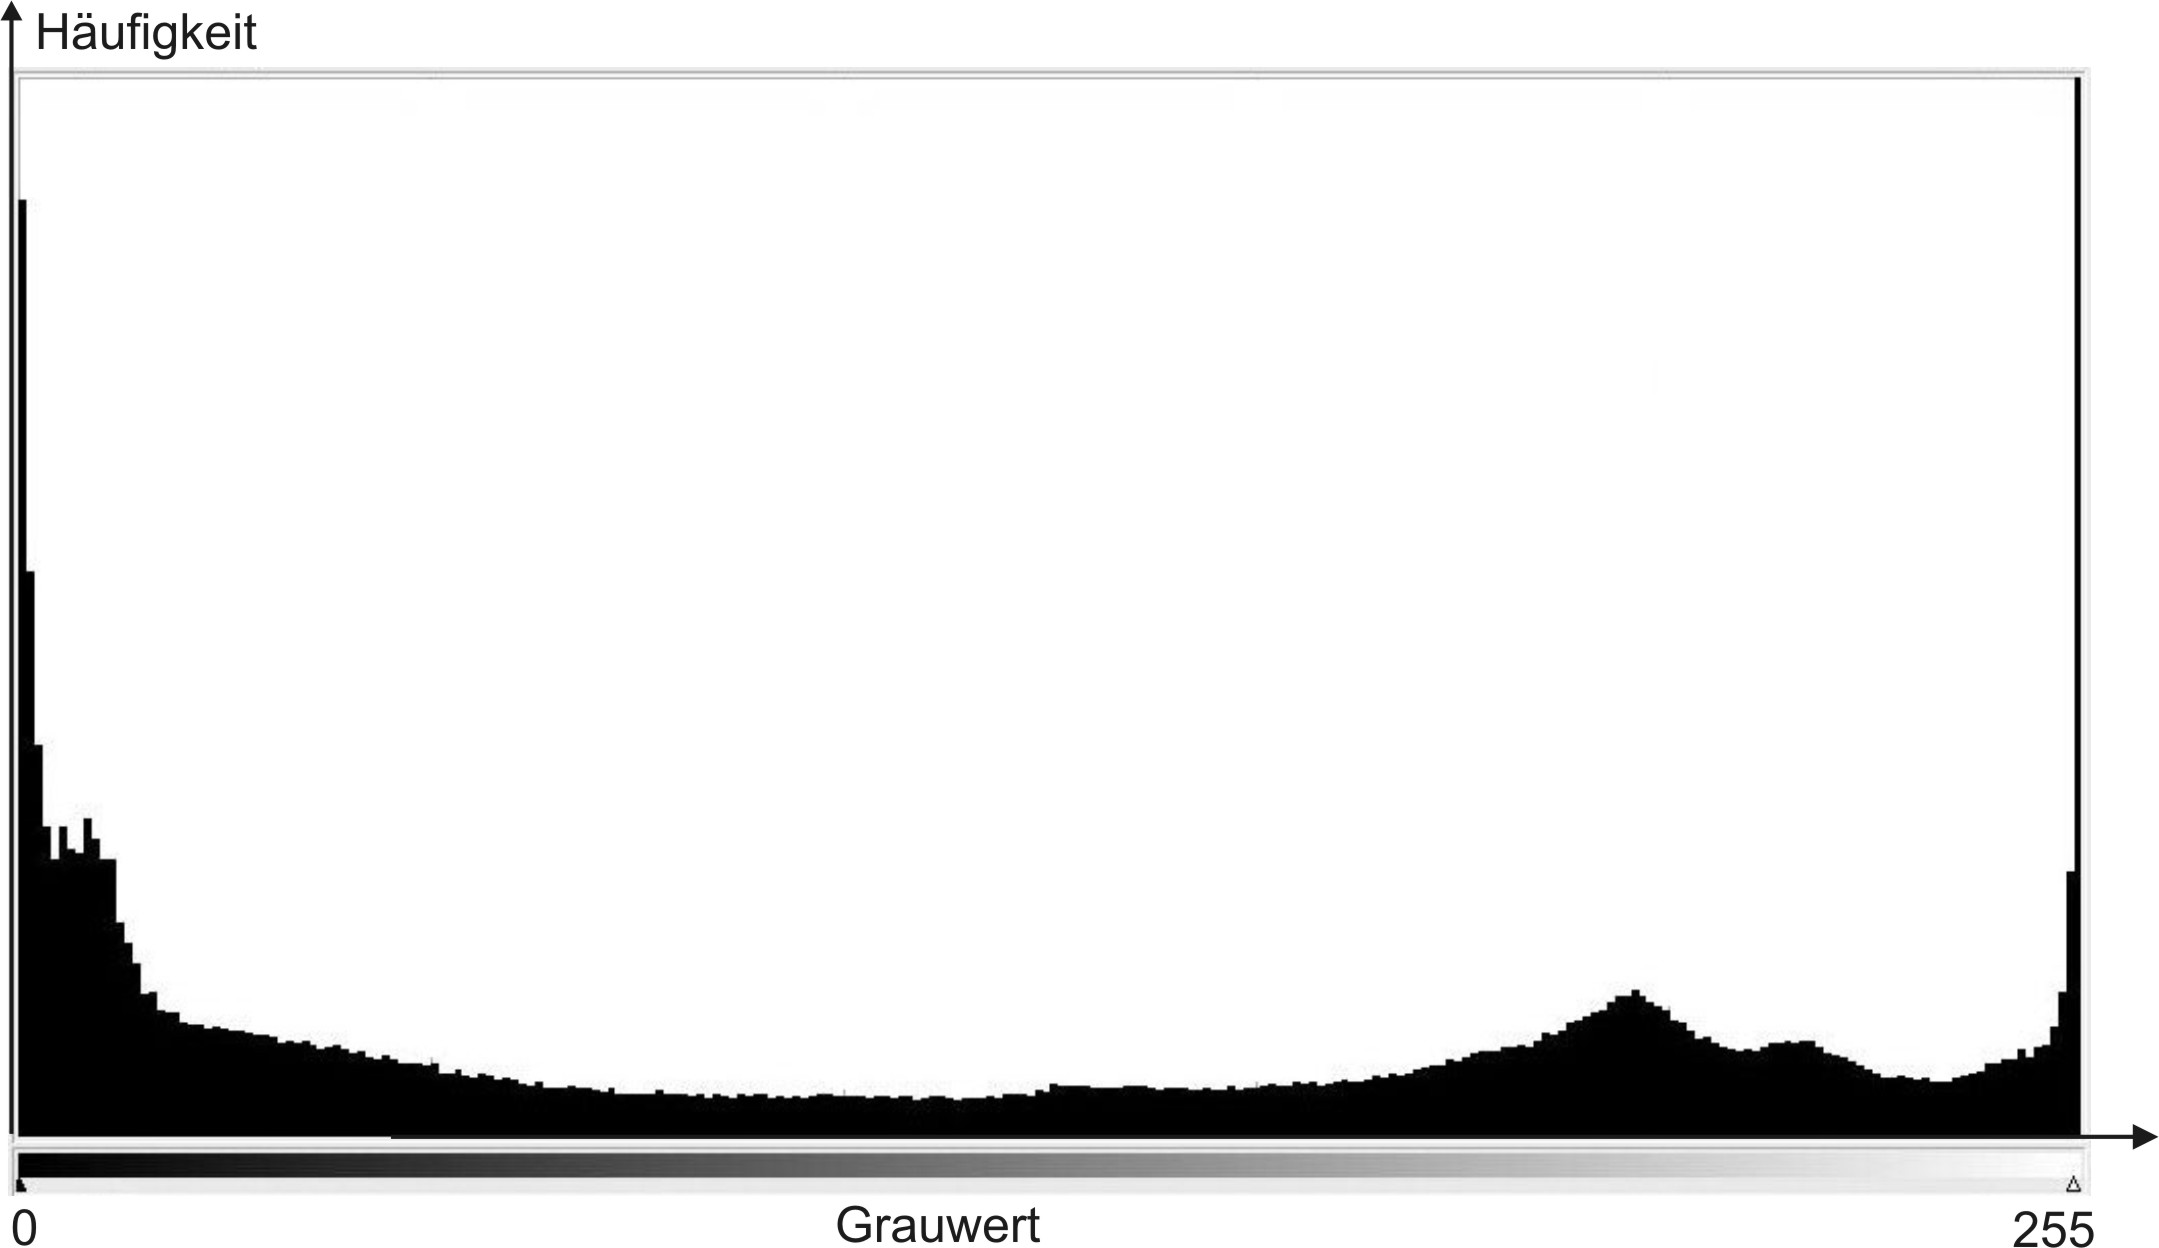
\includegraphics[scale=.5]{img/bildverarbeitung/histogramm.jpg}
	\end{tabular}
	\caption{Mel C in $514 \times 785$ Pixeln, $8$ Bit Auflösung und zugehöriges Histogramm}\label{melchisto}
\end{figure}

\subsection{Histogrammspreizung}
Die Histogrammspreizung (auch Tonwertspreizung genannt) ist ein häufig eingesetztes Verfahren zur Kontrastverstärkung in kontrastarmen Grauwertbildern. In solchen Bildern kommen viele Grauwerte der Grauwertskala überhaupt nicht vor. Je größer die ungenutzten Bereiche an den beiden Rändern der Skala sind, um so stärker kann der Abstand zwischen dem dunkelsten und dem hellsten Grauwert vergrößert werden, desto weiter können also die Grauwerte im Bild "`auseinandergezogen"' werden.\\
Durch eine lineare Skalierung wird die Grauwertverteilung eines Bildes $D$ über eine lineare Abbildung transformiert.
\begin{align}
D &\rightarrow D' \\
g'(i,j)&=(g(i,j)+c_1)\cdot c_2
\end{align}
Für $c_1 > 0$ wird das gesamte Bild heller, für $c_1 < 0$ dunkler. Die Konstante $c_2$
bewirkt eine Änderung des Kontrastes. Ein Wert größer~$1$ erhöht den Kontrast, für einen
Wert kleiner~$1$ wird das Bild kontrastärmer. Da der Grauwertbereich auf die Menge $G=\{0, \ldots, 255\}$
begrenzt ist, muss die oben angegebene Transformation noch so modifiziert werden, dass
die neuen Grauwerte von $D'$ innerhalb $G$ liegen.
\begin{align}
g'(i, j) &= \begin{cases} 0 &\text{falls} \, (g(i,j)+c_1)\cdot c_2 \leq 0 \\
255 &\text{falls} \, (g(i,j)+c_1)\cdot c_2 \geq 255\\
[(g(i,j)+c_1)\cdot c_2] &\text{sonst}
\end{cases}
\label{eq:histspreizung}
\end{align}
%\right
%$$

Hier sind die eckigen Klammern sogenannte Gaußklammern. Diese nehmen eine Rundung auf die
nächste natürliche Zahl vor. Durch die lineare Skalierung gehen dem Bild aber Information
verloren. In vielen Fällen handelt es sich dabei jedoch um nicht benötigte Information, die somit ausgeblendet werden kann.
Die optimalen Werte für $c_{1,2}$ können dem Histogramm entnommen werden. Dazu wird der 
minimale und maximale Grauwert im Bild bestimmt. Die Skalierungsparameter ergeben sich dann zu:
\begin{align}
c_1\,=&\, -\min\{g(i,j)\} \nonumber\\[1.5em]
c_2\,=&\, \frac{255}{\max\{g(i,j)\}-\min\{g(i,j)\}}\nonumber
\end{align}


\clearpage

\subsection{Histogrammegalisierung}
\label{sec:histo}
Die Histogrammegalisierung (auch Histogrammausgleich, Histogrammeinebnung oder Histogrammäqualisation genannt) ist ein wichtiges Verfahren zur Kontrastverbesserung in Grauwertbildern, das über eine bloße Kontrastverstärkung hinausgeht. Dabei wird aus der Grauwertverteilung im Histogramm eine Gleichverteilung berechnet, damit der gesamte zur Verfügung stehende Wertebereich optimal ausgenutzt wird. Diese Methode kommt besonders in solchen Fällen zur Anwendung, bei denen die interessanten Bildbereiche einen relativ großen Teil des Bildes ausmachen (die entsprechenden Grauwerte also überdurchschnittlich häufig vorkommen) und ihre Grauwerte auf einen kleinen Bereich der Grauwertskala begrenzt sind. Im Gegensatz zu einer Histogrammbegrenzung mit anschließender Histogrammspreizung, wo zwar der Kontrast im interessanten Grauwertbereich verstärkt wird, die Informationen außerhalb des Bereichs allerdings komplett verloren gehen, werden bei der Histogrammäqualisation häufige Grauwerte „auseinandergezogen“ (die Grauwertskala wird in diesen Bereichen gestreckt) und weniger häufige Grauwerte „zusammengeschoben“ (die Grauwertskala wird in diesen Bereichen gestaucht). Das Histogramm des Ergebnisbildes wird daher mehr oder weniger große Lücken enthalten (siehe Abbildung \ref{fig:histegal}). Dies begründet sich daraus, dass ein diskreter Grauwert auch nur auf einen anderen diskreten Grauwert abgebildet und nicht "`auseinandergezogen"' werden kann. Tritt ein Grauwert sehr häufig auf, so werden seine direkten "`Nachbarn"' auf der Grauwertskala nach der Gleichverteilung im Bild nicht mehr vorkommen.Als Basis zur Ermittlung der Transformationskennlinie dient das sogenannte kumulative Grauwerthistogramm $H_{k}$ des Bildes. Dieses wird berechnet, indem jedem Grauwert $g$ die Summe aller relativen Häufigkeiten $H$ der Grauwerte $0$ bis $g$ zugeordnet wird. Hierzu muss $H(n)$ als prozentuale Häufigkeit angegeben werden.
\begin{equation}
H_{k}(g)=\sum_{n=0}^{g}H(n)
\end{equation}
Dieses kumulative Grauwerthistogramm stellt eine Folge von Werten im Intervall $[0,1]$ dar. Durch Multiplikation jedes Elementes dieser Folge mit dem maximal möglichen Grauwert $G$, üblicherweise 255, und anschließender Rundung (eckige Klammern) ergibt sich die Transformationskennlinie mit Wertebereich $\lbrace0,\ldots,G\rbrace$:
\begin{equation}
T_{equal}(g)=\left\lbrack G\cdot H_k(g)\right\rbrack
\end{equation}
Diese Transformationskennlinie ordnet jedem Pixelgrauwert des Originalbildes einen Wert für das neue Bild zu.

Die Histogrammegalisierung ist verlustbehaftet, da größere Bereiche der Skala mit Grauwerten geringer Häufigkeit auf wenige Grauwerte komprimiert werden. Daher ist sie nicht umkehrbar\cite{histo}.

\begin{figure}[ht]
	\centering
	\begin{tabular}{cc}
		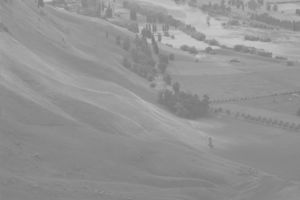
\includegraphics[width=0.45\textwidth]{img/bildverarbeitung/300px-Unequalized_Hawkes_Bay_NZ.jpg} & 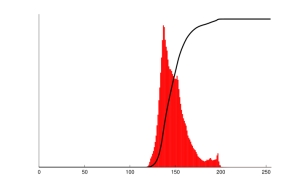
\includegraphics[width=0.45\textwidth]{img/bildverarbeitung/712px-Unequalized_Histogram.jpg} \\
		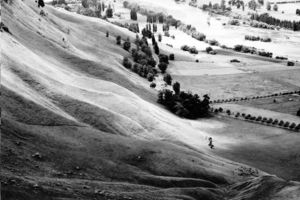
\includegraphics[width=0.45\textwidth]{img/bildverarbeitung/300px-Equalized_Hawkes_Bay_NZ.jpg} & 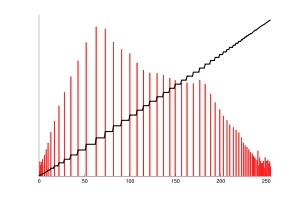
\includegraphics[width=0.45\textwidth]{img/bildverarbeitung/300px-Equalized_Histogram.jpg}
	\end{tabular}
	\caption[Beispiel einer Histogrammegalisierung]{Beispiel einer Histogrammegalisierung mit dazugehörigen Grauwertbildern. Die kumulativen Histogrammwerte sind schwarz, die "`gewöhnlichen"' Histogrammwerte rot dargestellt \cite{histo}.}
	\label{fig:histegal}
\end{figure}

\newpage

\subsection{Binäre Darstellung}
In einem FPGA, oder generell in Hardware, werden Zahlen mit Hilfe von Flip-Flops bzw. Register gespeichert. Im Gegensatz zu klassischen Programmiersprachen gibt es in einem FPGA jedoch keine Limitierung auf die gängigen Datentypen und deren Bitgrößen, sondern Bitsammlungenen in beliebiger Größe, da direkt auf Registerebene die Hardware beschrieben wird. Eine Herausforderung ist jedoch, dass durch die freie Repräsentation einer Zahl, während arithmetischen Berechnungen besonders auf Korrektheit und mögliche \emph{Überläufe}, beziehungsweise \emph{Unterläufe} geachtet werden muss.

\subsubsection{Darstellung im Dualsystem}
Wie der Name schon vermuten lässt, sind binäre Zahlen in Zweierpotenzen gespeichert (Vergleiche Vorlesung \emph{HMI}). Hierbei wird meist die Zahl mit dem größten Einfluss, genannt das MSB (most significant bit), an den Anfang und die Zahl mit dem kleinsten Einfluss, genannt das LSB (least significant bit), an das Ende geschrieben. Dies ist aber keineswegs ein Zwang, es sollte jedoch in einem Projekt einheitlich gearbeitet werden.

\begin{table}[H]
	\begin{center}
		\begin{tabular}{ccccccccccccccccccc}
			\textbf{MSB\textit{}} & 1 && 0 && 0 && 1 && 0 && 0 && 1 && 1 && \textbf{LSB\textit{}}& \\
			    & $2^7$ && $2^6$ && $2^5$ && $2^4$ && $2^3$ && $2^2$ && $2^1$ && $2^0$ &&& \\
			    & 128 & + & 0 & + & 0 & + & 16 & + & 0 & + & 0 & + & 2 & + & 1 &&& \textit{= 147}
		\end{tabular}
		\caption{Binäre Darstellung eines 8-bit Zahlenwertes}
		\label{tab:8bitnumber}
	\end{center}
\end{table}

Soll nun eine solche Zahl zurück in eine Dezimalzahl umwandelt werden, müssen nur die einzelnen Bitwerte addiert werden. Ein solcher Bitwert ergibt sich aus $2^x$, wobei $x$ die Position des Bits vom LSB nach links gezählt ist. Dies ergibt eine Summenformel, die aus der Mathematikvorlesung bekannt ist:
\begin{align}
	n = \sum_{x=0}^{X-1}b[x] \cdot 2^x
\end{align}
Wobei $b$ ein Bitarray einer binären Zahl mit der Größe $X$ ist.

\subsubsection{Addition}
Die Binäre Addition funktioniert prinzipiell genauso, wie schriftliche Addition, nur zur Basis 2.

Die Addition beginnt mit dem LSBs der Zahlen. \textbf{0} und \textbf{0} ergibt \textbf{0}, \textbf{0} und \textbf{1} ergibt \textbf{1}, \textbf{1} und \textbf{1} ergibt \textbf{10}. Letzteres ergibt also \textbf{0} mit Übertrag \textbf{1}. \\
Dies ist bekannt aus der Mikroelektronik Vorlesung (Halfadder, Fulladder, Carrybit).\\

\textbf{Beispiel:} (Addition von 001111 und 101010)\\ \\
\begin{tabular}{ccccccccc}
	 &0&0&1&1&1&0&0&1\\
	+&1&0&1&0&1&0&1&1\\
	\hline
	&&\scriptsize{1}&\scriptsize{1}&\scriptsize{1}&&\scriptsize{1}&\scriptsize{1}& \\
	\hline
	&\textbf{1}&\textbf{1}&\textbf{1}&\textbf{0}&\textbf{0}&\textbf{1}&\textbf{0}&\textbf{0}
\end{tabular}

\subsubsection{Multiplikation}
Auch die Multiplikation ist kein Hexenwerk und funktioniert genauso wie die schriftliche Multiplikation. Eine der beiden Zahlen wird bitweise durchlaufen und jeweils mit der gesamten anderen Zahl multipliziert. Alle Ergebnisse werden anschließend addiert.
\newpage
Der Übersicht halber werden im Beispiel 4-bit Zahlen verwendet.\\

\textbf{Beispiel:} (Multiplikation von 1101 und 1001)\\ 
\begin{tabular}{cccccccccc}
	&1&1&0&1&$\cdot$&1&0&0&1\\
	\hline
	 &&&&&&1&1&0&1\\
	+&&&&&0&0&0&0&\\
	+&&&&0&0&0&0&&\\
	+&&&1&1&0&1&&&\\
	\hline
	 &&&\textbf{1}&\textbf{1}&\textbf{1}&\textbf{0}&\textbf{1}&\textbf{0}&\textbf{1}
\end{tabular}

\subsubsection{Binäre Darstellung von reellen Zahlen}
Ganze Zahlen lassen sich sehr einfach mittels Binärdarstellung abbilden. Sollen jedoch reelle Zahlen gespeichert werden, sieht das ganze jedoch etwas anders aus.

\textbf{Festkommazahlen}:\\
Die einfachste Methode Kommazahlen abzuspeichern ist es eine gewisse Bitlänge für den Bereich vor und hinter dem Komma zu definieren und somit eine Zahl mit Nachkommastelle zu erhalten. Auch wenn eine Division auf diese Art und Weise deutlich einfacher zu realisieren ist als bei Gleikommazahlen, hat die Festkommazahl den entscheidenden Nachteil, dass der Wertebereich beschränkt ist.

Ein entscheidender Vorteil von Festkommazahlen ist jedoch, dass sich Addition und Multiplikation genauso verhalten, wie bei Integerzahlen. Es müssen nur zusätzlich die Nachkommastellen beachtet werden.\\
Im kommenden Beispiel nehmen wir jeweils 4 Bit für die Vorkomma-, sowie Nachkommastellen an.\\

\textbf{Beispiel:} (Multiplikation) \\
\begin{tabular}{cccccc}
	dezimal: & 3,5 & $\cdot$ & 2,5 & = & 8,75 \\
	binär: & 0011,1000 & $\cdot$ & 0010,1000 & = & 0001000,11000000 \\
\end{tabular}\\
\\ \\
Die Verschiebung der Nachkommastellen ist sowohl dezimal als auch binär des Ergebnis die Addition der Verschiebung der beiden Eingangswerte. \\
Im Rahmen des Praktikums werden Festkommazahlen verwendet.
\\

\textbf{Gleitkommazahlen}:\\
Im Gegensatz zu den Festkommazahlen sind die Gleitkommazahlen nicht als zwei Integer mit einem Trennungskomma gespeichert, sondern etwas dynamischer.

Eine Gleitkommazahl ist wie folgt aufgebaut: $Mantisse$ $\cdot$ $Basis^{Exponent}$. (Beispiel: $1456 \cdot 10^{-3} = 1,456$)

Im IEEE-Format besteht die Mantisse aus den ersten 23 Bits (32 bit), beziehungsweise den ersten 52 Bits (64 bit). Das letzte Bit wird für das Vorzeichen der Zahl verwendet und die restlichen Bits für den Exponenten. Aber auch der Exponent hat ein Vorzeichen. Hat dieser 8 Bit, so reicht der Exponent von -128 bis 127. Dadurch wird gewährleistet, dass die Mantisse eine Ganzzahl sein kann, die durch die Multiplikation einer Exponentialfunktion Werte in einem sehr großem Spektrum annehmen kann ($1 \cdot 10^{-128}$ bis $999...9 \cdot 10^{127}$).

\textbf{Beispiel:} (32-bit Zahl 01101101001100101010010101011101)\\
\begin{tabular}{ccc}
0 & 11011010 & 01100101010010101011101\\
\textbf{Vorzeichen} & \textbf{Exponent} & \textbf{Mantisse}
\\
+ & $10^{-90}$ & 3319133
\end{tabular}

Beachten Sie, dass hier das MSB des Exponenten das Vorzeichen beinhaltet.\cite{floating_point}
\subsection{\textsc{Versuch 2 und Aufgaben}}
Siehe Dokument zur Aufgabenstellung Kapitel 2.
\newpage

